\subsection{Session 2, Exercise 2}

\lineparagraph{Exercise}

Let $\Sigma=\{0,1\}$. Give a deterministic finite automaton that accepts the words that contain an even number of zeroes, while the number of ones is divisible by three.

\lineparagraph{Solution}


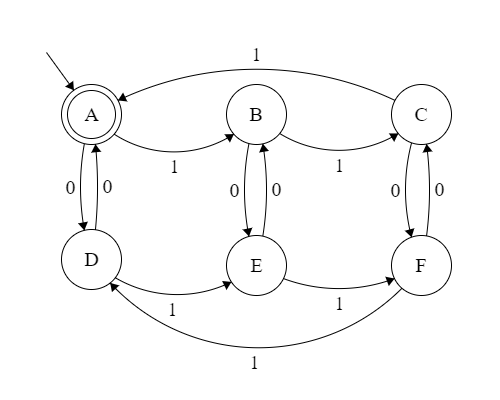
\includegraphics[width=0.5\linewidth]{02/2_2.png}

Proof:

Let's look at what the states mean:

\begin{itemize}
    \item A: State $A$ represents words that contain an even number of $0$'s and the number of $1$'s is in the form $3k$ (divisible by three).
    \item B: State $B$ represents words that contain an even number of $0$'s and the number of $1$'s is in the form $3k+1$.
    \item C: State $C$ represents words that contain an even number of $0$'s and the number of $1$'s is in the form $3k+2$.
    \item D: State $D$ represents words that contain an odd number of $0$'s and the number of $1$'s is in the form $3k$ (divisible by three).
    \item E: State $E$ represents words that contain an odd number of $0$'s and the number of $1$'s is in the form $3k+1$.
    \item F: State $F$ represents words that contain an odd number of $0$'s and the number of $1$'s is in the form $3k+2$.
\end{itemize}

Let's look at the starting state and the accepting and rejecting states:

\begin{itemize}
    \item The starting state is the state that should represent the empty string. The empty string contains zero $0$'s and zero $1$'s, and zero is even and also divisible by three, which is represented by $A$, so the starting state is $A$.
    \item The only accepting state is $A$, since we want to accept words that contain an even number of zeros and the number of ones is divisible by three in them, which are represented by $A$.
    \item The other states are rejecting states, since they represent words that are not in the desired language.
\end{itemize}

Let's look at the transitions:

\begin{itemize}
    \item Transitions triggered by a $0$ input are $A\rightarrow{}D$, $D\rightarrow{}A$, $B\rightarrow{}E$, $E\rightarrow{}B$, $C\rightarrow{}F$, $F\rightarrow{}C$. In these cases the parity of the $1$'s doesn't change, while the parity of the $0$'s is inverted. If we look back on what the states represent we can verify in all $6$ cases that this is the case.
    \item Transitions triggered by a $1$ input:
    \begin{itemize}
        \item $A\rightarrow{}B$ and $D\rightarrow{}E$ move from states that have seen $3k$ $1$'s to states that have sen $3k+1$ $1$'s (the remainder goes from $0$ to $1$).
        \item $B\rightarrow{}C$ and $E\rightarrow{}F$ move from states that have seen $3k+1$ $1$'s to states that have sen $3k+2$ $1$'s (the remainder goes from $1$ to $2$).
        \item $C\rightarrow{}A$ and $F\rightarrow{}D$ move from states that have seen $3k+2$ $1$'s to states that have sen $3k$ $1$'s (the remainder goes from $2$ to $0$).
    \end{itemize}
\end{itemize}